\documentclass[../../../main.tex]{subfiles}

\begin{document}

\section{Fundamental Theorems}

There are many foundational topics and theorems to discuss.
Before we get into more advanced topics, let's discuss key theorems
like Pascal's theorem and Desargues' theorem.

\subsection{Pascal's Theorem}

Let's first get started with Pascal's theorem! Surprisingly,
Pascal's theorem is considered a topic in projective geometry even if
it holds in Euclidean plane for some case because parallel pairs
deal with point at infinity. Here is the statement.

\begin{theorem}{Pascal's Theorem}{Pascal's Theorem}
Given six points $A, B, C, D, E, F$ on a conic section,
if $X = AB \cap DE$, $Y = CD \cap FA$, and $Z = EF \cap BC$,
then $X, Y, Z$ are collinear, whose line is known as
\textbf{Pascal line}.
\end{theorem}

We stated here as conic section, but we can just consider it as a
circle because majority of the problems deal with circle. Also,
one tip for memorizing the definition of $X, Y, Z$ is the following.
\[
\begin{NiceArray}{cc|cc|cc}
    A & B & C & D & E & F \\
    D & E & F & A & B & C
\end{NiceArray}
\]
Sometimes it is easy to mess up like $AD \cap BE$, but remembering
$AB$ helped for me. Also, there are few different diagrams when you
search Pascal's theorem depending on the orientation of the hexagon,
but here is the famous and clean diagram.

\begin{figure}[H]
\centering
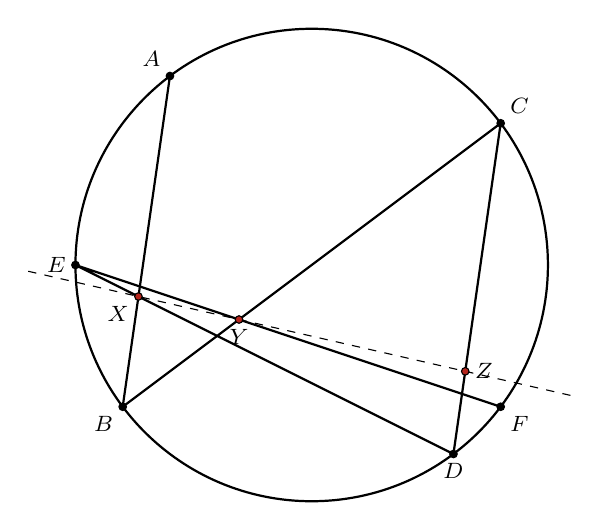
\begin{tikzpicture}[scale=0.6]
    \coordinate (A) at (-3,4);
    \coordinate (B) at (-4,-3);
    \coordinate (C) at (4,3);
    \coordinate (D) at (3,-4);
    \coordinate (E) at (-5,0);
    \coordinate (F) at (4,-3);
    \coordinate (X) at (-3.666666666666666,-0.6666666666666669);
    \coordinate (Y) at (-1.5384615384615385,-1.1538461538461537);
    \coordinate (Z) at (3.25,-2.25);
    \coordinate (P) at (7,-6);
    \coordinate (Q) at (-2,-1.5);
    \coordinate (R) at (0.5714285714285721,0.428571428571429);

    \draw[thick] (0, 0) circle (5);

    \draw[thick] (A) -- (B) -- (C) -- (D) -- (E) -- (F);
    \draw[dashed]
        (-6,-0.13253012048192805) -- (5.5,-2.7650602409638547);

    \draw[fill=black] (A) circle (0.08)
        node[above left] {\footnotesize $A$};
    \draw[fill=black] (B) circle (0.08)
        node[below left] {\footnotesize $B$};
    \draw[fill=black] (C) circle (0.08)
        node[above right] {\footnotesize $C$};
    \draw[fill=black] (D) circle (0.08)
        node[below] {\footnotesize $D$};
    \draw[fill=black] (E) circle (0.08)
        node[left] {\footnotesize $E$};
    \draw[fill=black] (F) circle (0.08)
        node[below right] {\footnotesize $F$};
    \draw[fill=BrickRed] (X) circle (0.08)
        node[below left] {\footnotesize $X$};
    \draw[fill=BrickRed] (Y) circle (0.08)
        node[below] {\footnotesize $Y$};
    \draw[fill=BrickRed] (Z) circle (0.08)
        node[right] {\footnotesize $Z$};
\end{tikzpicture}
\end{figure}

There are many different ways to prove this theorem, and I think the
most popular method is using Menelaus. However, there are also many
different interesting ways of proving this, so let's prove Pascal's
theorem using two different ways.

\begin{proof}
The first proof involves using Menelaus three times. First,
consider the new points $P, Q, R$.

\begin{figure}[H]
\centering
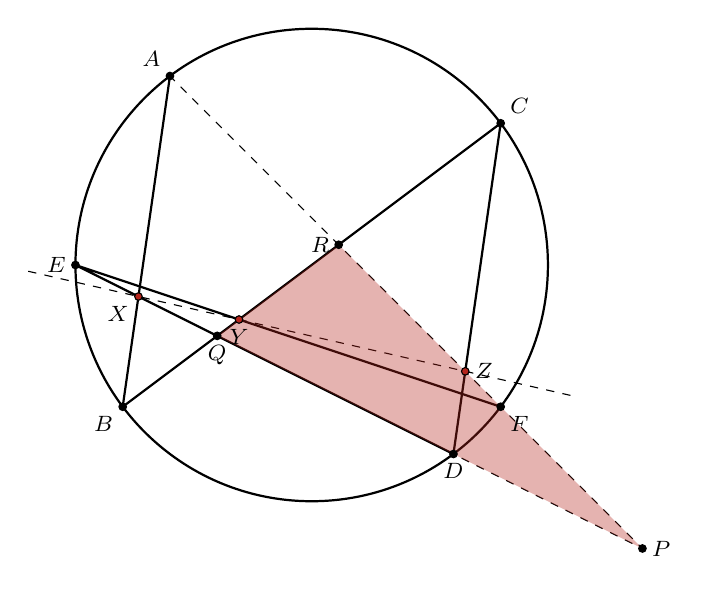
\begin{tikzpicture}[scale=0.6]
    \coordinate (A) at (-3,4);
    \coordinate (B) at (-4,-3);
    \coordinate (C) at (4,3);
    \coordinate (D) at (3,-4);
    \coordinate (E) at (-5,0);
    \coordinate (F) at (4,-3);
    \coordinate (X) at (-3.666666666666666,-0.6666666666666669);
    \coordinate (Y) at (-1.5384615384615385,-1.1538461538461537);
    \coordinate (Z) at (3.25,-2.25);
    \coordinate (P) at (7,-6);
    \coordinate (Q) at (-2,-1.5);
    \coordinate (R) at (0.5714285714285721,0.428571428571429);

    \draw[thick] (0, 0) circle (5);

    \draw[thick] (A) -- (B) -- (C) -- (D) -- (E) -- (F);
    \draw[dashed]
        (-6,-0.13253012048192805) -- (5.5,-2.7650602409638547);
    \draw[dashed] (E) -- (P) -- (A);
    \fill[BrickRed, opacity=0.35] (P) -- (Q) -- (R) -- cycle;

    \draw[fill=black] (A) circle (0.08)
        node[above left] {\footnotesize $A$};
    \draw[fill=black] (B) circle (0.08)
        node[below left] {\footnotesize $B$};
    \draw[fill=black] (C) circle (0.08)
        node[above right] {\footnotesize $C$};
    \draw[fill=black] (D) circle (0.08)
        node[below] {\footnotesize $D$};
    \draw[fill=black] (E) circle (0.08)
        node[left] {\footnotesize $E$};
    \draw[fill=black] (F) circle (0.08)
        node[below right] {\footnotesize $F$};
    \draw[fill=BrickRed] (X) circle (0.08)
        node[below left] {\footnotesize $X$};
    \draw[fill=BrickRed] (Y) circle (0.08)
        node[below] {\footnotesize $Y$};
    \draw[fill=BrickRed] (Z) circle (0.08)
        node[right] {\footnotesize $Z$};
    \draw[fill=black] (P) circle (0.08)
        node[right] {\footnotesize $P$};
    \draw[fill=black] (Q) circle (0.08)
        node[below] {\footnotesize $Q$};
    \draw[fill=black] (R) circle (0.08)
        node[left] {\footnotesize $R$};
\end{tikzpicture}
\end{figure}

From the triangle $PQR$, the following equations can be obtained with
Menelaus' theorem.
\begin{align*}
    \frac{PA}{AR} \cdot \frac{RB}{BQ} \cdot \frac{QX}{XP} &= 1 \\
    \frac{PZ}{ZR} \cdot \frac{RC}{CQ} \cdot \frac{QD}{DP} &= 1 \\
    \frac{EQ}{PE} \cdot \frac{YR}{QY} \cdot \frac{FP}{RF} &= 1
\end{align*}
Moreover by Power of a Point theorem, the following equations hold.
\begin{align*}
    PD \cdot PE &= PF \cdot PA \\
    BQ \cdot QC &= EQ \cdot QD \\
    BR \cdot RC &= AR \cdot RF
\end{align*}
Multiplying the equations,
\[
\frac{QX}{XP} \cdot \frac{PZ}{ZR} \cdot \frac{YR}{QY} = 1
\]
is obtained and $X, Y, Z$ are collinear by Menelaus' theorem.
\end{proof}

The next one is less popular, but also an interesting proof.

\begin{proof}
First, consider the following annotated diagram.

\begin{figure}[H]
\centering
\begin{tikzpicture}[scale=0.6]
    \coordinate (A) at (-3,4);
    \coordinate (B) at (-4,-3);
    \coordinate (C) at (4,3);
    \coordinate (D) at (3,-4);
    \coordinate (E) at (-5,0);
    \coordinate (F) at (4,-3);
    \coordinate (X) at (-3.666666666666666,-0.6666666666666669);
    \coordinate (Y) at (-1.5384615384615385,-1.1538461538461537);
    \coordinate (Z) at (3.25,-2.25);
    \coordinate (P) at (-1.0769230769230766,2.076923076923078);
    \coordinate (Q) at (3.0769230769230775,-3.4615384615384612);

    \draw[thick] (0, 0) circle (5);
    \draw[thick, BrickRed]
        (1.9230769230769231,0) circle (3.6487819155788994);

    \draw[thick] (A) -- (B) -- (C) -- (D) -- (E) -- (F);
    \draw[dashed]
        (-6,-0.13253012048192805) -- (5.5,-2.7650602409638547);
    \draw[thick] (A) -- (D);
    \draw[thick] (P) -- (Y);
    \draw[thick] (P) -- (Q);
    \draw[thick] (F) -- (P);
    \draw[thick] (A) -- (P);

    \fill[BrickRed, opacity=0.35] (A) -- (X) -- (D) -- cycle;
    \fill[RoyalPurple, opacity=0.35] (P) -- (Y) -- (Q) -- cycle;

    \draw[fill=black] (A) circle (0.08)
        node[above left] {\footnotesize $A$};
    \draw[fill=black] (B) circle (0.08)
        node[below left] {\footnotesize $B$};
    \draw[fill=black] (C) circle (0.08)
        node[above right] {\footnotesize $C$};
    \draw[fill=black] (D) circle (0.08)
        node[below] {\footnotesize $D$};
    \draw[fill=black] (E) circle (0.08)
        node[left] {\footnotesize $E$};
    \draw[fill=black] (F) circle (0.08)
        node[below right] {\footnotesize $F$};
    \draw[fill=BrickRed] (X) circle (0.08)
        node[below left] {\footnotesize $X$};
    \draw[fill=BrickRed] (Y) circle (0.08)
        node[below] {\footnotesize $Y$};
    \draw[fill=BrickRed] (Z) circle (0.08)
        node[right] {\footnotesize $Z$};
    \draw[fill=black] (P) circle (0.08)
        node[right] {\footnotesize $P$};
    \draw[fill=black] (Q) circle (0.08)
        node[below right] {\footnotesize $Q$};

    \pic[draw,"$\circ$", angle radius=8mm, angle eccentricity=1.4]
        {angle=X--A--D};
    \pic[draw,"$\circ$", angle radius=8mm, angle eccentricity=1.4]
        {angle=Y--P--Q};
    \pic[draw,"$\bullet$", angle radius=8mm, angle eccentricity=1.4]
        {angle=A--D--X};
    \pic[draw,"$\bullet$", angle radius=8mm, angle eccentricity=1.4]
        {angle=P--Q--Y};
    \pic[draw,"$\times$", angle radius=12mm, angle eccentricity=1.4]
        {angle=D--A--F};
    \pic[draw,"$\times$", angle radius=12mm, angle eccentricity=1.4]
        {angle=Q--P--F};
\end{tikzpicture}
\end{figure}

First, notice that $\angle{FPQ} = \angle{DCF} = \angle{DAF}$.
Therefore, $AD \parallel PQ$. Similarly, $\angle{XAD} = \angle{BCD}
= \angle{YPQ}$ and $\angle{ADX} \angle{AFE} = \angle{PTQ}$. Therefore,
$\triangle{AXD} \sim \triangle{PYQ}$. Moreover, because $Z$ is the
center of homothety, $X, Y, Z$ lie on the same line.
\end{proof}

Pascal's theorem is arguably one of more popular and foundational
theorem in olympiad geometry. With the idea in mind, here is a
practice problem.

\begin{problem}{}{}
PASCAL PROBLEM
\end{problem}



\subsection{Desargues' Theorem}

Continuing from Pascal's theorem, here is Desargues' theorem.

\begin{theorem}{Desargues' Theorem}{Desargues' Theorem}
Two triangles are axially perspective if and only if they are
centrally perspective. Two triangles are considered axially
perspective if there exists the axis of perspectivity and they are
centrally perspective if there exists the center of perspectivity.
\end{theorem}

For simpler explanation, consider the diagram below, which is simply
the extension of Figure \ref{fig:Desargues Theorem Figure 1}.

\begin{figure}[H]
\centering
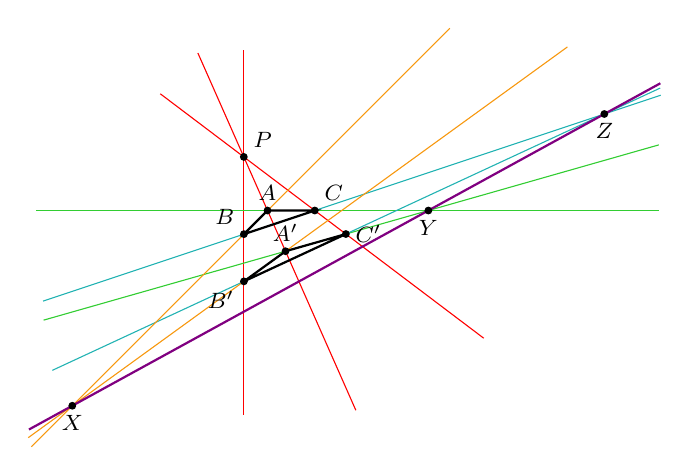
\begin{tikzpicture}[scale=0.06]
    \coordinate (A) at (5, 15);
    \coordinate (B) at (0, 10);
    \coordinate (C) at (15, 15);
    \coordinate (A') at (8.81, 6.384);
    \coordinate (B') at (0, 0);
    \coordinate (C') at (21.585, 10.024);
    \coordinate (P) at (-0.018, 26.349);
    \coordinate (X) at (-36.326, -26.326);
    \coordinate (Y) at (39.052, 15);
    \coordinate (Z) at (76.3, 35.433);

    \draw[red] (-17.695, 39.707) -- (50.757, -12.021);
    \draw[red] (-9.742, 48.339) -- (23.695, -27.279);
    \draw[red] (0, 48.926) -- (0, -28.305);

    \draw[LimeGreen] (-43.959, 15) -- (87.893, 15);
    \draw[LimeGreen] (-42.399, -8.204) -- (87.824, 28.894);
    \draw[TealBlue] (-42.509, -4.17) -- (88.226, 39.409);
    \draw[TealBlue] (-40.544, -18.828) -- (88.117, 40.921);
    \draw[YellowOrange]
        (-45.653, -33.086) -- (68.479, 49.628);
    \draw[YellowOrange]
        (-45, -35) -- (43.588, 53.588);

    \draw[thick, violet]
        (-45.498, -31.355) -- (88.156, 41.935);

    \draw[thick] (A) -- (B) -- (C) -- (A);
    \draw[thick] (A') -- (B') -- (C') -- (A');

    \foreach \n in {A, B, C, A', B', C', X, Y, Z, P}
    \node at (\n)[circle,fill,inner sep=1pt]{};

    \node[above] at (A) {\footnotesize $A$};
    \node[above left] at (B) {\footnotesize $B$};
    \node[above right] at (C) {\footnotesize $C$};
    \node[above] at (A') {\footnotesize $A'$};
    \node[below left] at (B') {\footnotesize $B'$};
    \node[right] at (C') {\footnotesize $C'$};
    \node[above right] at (P) {\footnotesize $P$};
    \node[below] at (X) {\footnotesize $X$};
    \node[below] at (Y) {\footnotesize $Y$};
    \node[below] at (Z) {\footnotesize $Z$};
\end{tikzpicture}
\label{fig:Figure 2}
\end{figure}

Point $P$, where $AA', BB', CC'$ concur, is the center of
perspectivity. Line $XZ$, where $X, Y, Z$ are collinear, is the axis
of perspectivity in the diagram above. If the pairs of corresponding
lines are all parallel, it is said that the lines meet at a point of
infinity. However, we normally don't discuss about that case.

The theorem is stating that if there exists a point $P$ such that
$P = AA' \cap BB' \cap CC'$, then the points $X = AB \cap A'B'$,
$Y = BC \cap B'C'$, and $Z = CA \cap C'A'$ are collinear.
With this in mind, let's try to prove the theorem.

\begin{proof}
The proof of the theorem involves the use of Menelaus' theorem three
times \cite{MATH01-1}. First, let's prove that two triangles are
axially perspective if they are centrally perspective.

Assuming that $\triangle{ABC}$ and $\triangle{A'B'C'}$ are perspective
from point $P$, Menelaus' Theorem can be applied.

\begin{center}
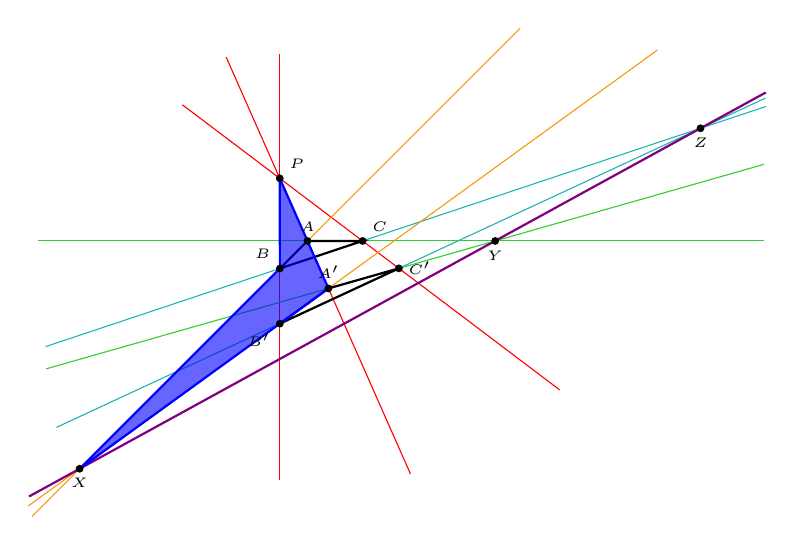
\begin{tikzpicture}[scale=0.07]
    \coordinate (A) at (5, 15);
    \coordinate (B) at (0, 10);
    \coordinate (C) at (15, 15);
    \coordinate (A') at (8.81, 6.384);
    \coordinate (B') at (0, 0);
    \coordinate (C') at (21.585, 10.024);
    \coordinate (P) at (-0.018, 26.349);
    \coordinate (X) at (-36.326, -26.326);
    \coordinate (Y) at (39.052, 15);
    \coordinate (Z) at (76.3, 35.433);

    \draw[red] (-17.695, 39.707) -- (50.757, -12.021);
    \draw[red] (-9.742, 48.339) -- (23.695, -27.279);
    \draw[red] (0, 48.926) -- (0, -28.305);

    \draw[LimeGreen] (-43.959, 15) -- (87.893, 15);
    \draw[LimeGreen] (-42.399, -8.204) -- (87.824, 28.894);
    \draw[TealBlue] (-42.509, -4.17) -- (88.226, 39.409);
    \draw[TealBlue] (-40.544, -18.828) -- (88.117, 40.921);
    \draw[YellowOrange]
        (-45.653, -33.086) -- (68.479, 49.628);
    \draw[YellowOrange]
        (-45, -35) -- (43.588, 53.588);

    \draw[thick, violet]
        (-45.498, -31.355) -- (88.156, 41.935);

    \draw[thick] (A) -- (B) -- (C) -- (A);
    \draw[thick] (A') -- (B') -- (C') -- (A');
    \draw[thick, blue]
        (P) -- (A) -- (A') -- (X) -- (B) -- (P);

    \fill[blue, opacity=0.6]
        (P) -- (A) -- (A') -- (X) -- (B);

    \foreach \n in {A, B, C, A', B', C', X, Y, Z, P}
        \node at (\n)[circle,fill,inner sep=1pt]{};

    \node[above] at (A) {\tiny $A$};
    \node[above left] at (B) {\tiny $B$};
    \node[above right] at (C) {\tiny $C$};
    \node[above] at (A') {\tiny $A'$};
    \node[below left] at (B') {\tiny $B'$};
    \node[right] at (C') {\tiny $C'$};
    \node[above right] at (P) {\tiny $P$};
    \node[below] at (X) {\tiny $X$};
    \node[below] at (Y) {\tiny $Y$};
    \node[below] at (Z) {\tiny $Z$};
\end{tikzpicture}
\end{center}
Consider $\triangle{PA'B'}$ with transverse line $XB$. Using Menelaus'
Theorem, the following equation could be derived.
\[
\frac{XA'}{XB'} \cdot \frac{BB'}{BP} \cdot \frac{AP}{AA'}
= 1
\]
\begin{center}
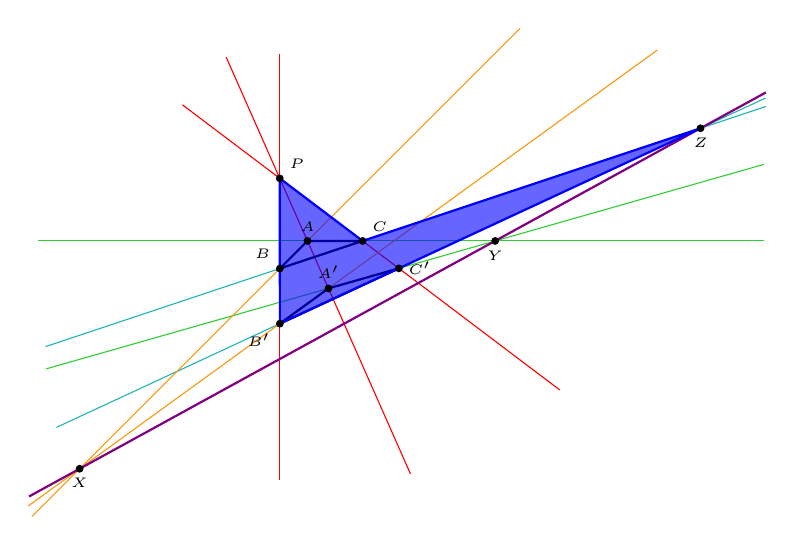
\begin{tikzpicture}[scale=0.07]
    \coordinate (A) at (5, 15);
    \coordinate (B) at (0, 10);
    \coordinate (C) at (15, 15);
    \coordinate (A') at (8.81, 6.384);
    \coordinate (B') at (0, 0);
    \coordinate (C') at (21.585, 10.024);
    \coordinate (P) at (-0.018, 26.349);
    \coordinate (X) at (-36.326, -26.326);
    \coordinate (Y) at (39.052, 15);
    \coordinate (Z) at (76.3, 35.433);

    \draw[red] (-17.695, 39.707) -- (50.757, -12.021);
    \draw[red] (-9.742, 48.339) -- (23.695, -27.279);
    \draw[red] (0, 48.926) -- (0, -28.305);

    \draw[LimeGreen] (-43.959, 15) -- (87.893, 15);
    \draw[LimeGreen] (-42.399, -8.204) -- (87.824, 28.894);
    \draw[TealBlue] (-42.509, -4.17) -- (88.226, 39.409);
    \draw[TealBlue] (-40.544, -18.828) -- (88.117, 40.921);
    \draw[YellowOrange]
        (-45.653, -33.086) -- (68.479, 49.628);
    \draw[YellowOrange]
        (-45, -35) -- (43.588, 53.588);

    \draw[thick, violet]
        (-45.498, -31.355) -- (88.156, 41.935);

    \draw[thick] (A) -- (B) -- (C) -- (A);
    \draw[thick] (A') -- (B') -- (C') -- (A');
    \draw[thick, blue]
        (P) -- (B') -- (C') -- (Z) -- (C) -- (P);

    \fill[blue, opacity=0.6]
        (P) -- (B') -- (C') -- (Z) -- (C);

    \foreach \n in {A, B, C, A', B', C', X, Y, Z, P}
        \node at (\n)[circle,fill,inner sep=1pt]{};

    \node[above] at (A) {\tiny $A$};
    \node[above left] at (B) {\tiny $B$};
    \node[above right] at (C) {\tiny $C$};
    \node[above] at (A') {\tiny $A'$};
    \node[below left] at (B') {\tiny $B'$};
    \node[right] at (C') {\tiny $C'$};
    \node[above right] at (P) {\tiny $P$};
    \node[below] at (X) {\tiny $X$};
    \node[below] at (Y) {\tiny $Y$};
    \node[below] at (Z) {\tiny $Z$};
\end{tikzpicture}
\end{center}
Similarly, consider $\triangle{PB'C'}$ and transverse line $ZC$.
\[
\frac{ZB'}{ZC'} \cdot \frac{CC'}{CP} \cdot \frac{BP}{BB'}
= 1
\]
\begin{center}
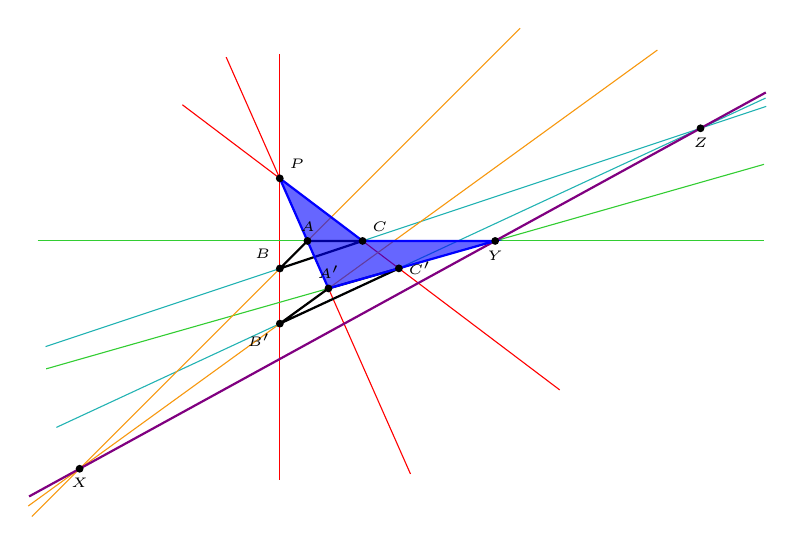
\begin{tikzpicture}[scale=0.07]
    \coordinate (A) at (5, 15);
    \coordinate (B) at (0, 10);
    \coordinate (C) at (15, 15);
    \coordinate (A') at (8.81, 6.384);
    \coordinate (B') at (0, 0);
    \coordinate (C') at (21.585, 10.024);
    \coordinate (P) at (-0.018, 26.349);
    \coordinate (X) at (-36.326, -26.326);
    \coordinate (Y) at (39.052, 15);
    \coordinate (Z) at (76.3, 35.433);

    \draw[red] (-17.695, 39.707) -- (50.757, -12.021);
    \draw[red] (-9.742, 48.339) -- (23.695, -27.279);
    \draw[red] (0, 48.926) -- (0, -28.305);

    \draw[LimeGreen] (-43.959, 15) -- (87.893, 15);
    \draw[LimeGreen] (-42.399, -8.204) -- (87.824, 28.894);
    \draw[TealBlue] (-42.509, -4.17) -- (88.226, 39.409);
    \draw[TealBlue] (-40.544, -18.828) -- (88.117, 40.921);
    \draw[YellowOrange]
        (-45.653, -33.086) -- (68.479, 49.628);
    \draw[YellowOrange]
        (-45, -35) -- (43.588, 53.588);

    \draw[thick, violet]
        (-45.498, -31.355) -- (88.156, 41.935);

    \draw[thick] (A) -- (B) -- (C) -- (A);
    \draw[thick] (A') -- (B') -- (C') -- (A');
    \draw[thick, blue]
        (P) -- (A') -- (C') -- (Y) -- (C) -- (P);

    \fill[blue, opacity=0.6]
        (P) -- (A') -- (C') -- (Y) -- (C);

    \foreach \n in {A, B, C, A', B', C', X, Y, Z, P}
        \node at (\n)[circle,fill,inner sep=1pt]{};

    \node[above] at (A) {\tiny $A$};
    \node[above left] at (B) {\tiny $B$};
    \node[above right] at (C) {\tiny $C$};
    \node[above] at (A') {\tiny $A'$};
    \node[below left] at (B') {\tiny $B'$};
    \node[right] at (C') {\tiny $C'$};
    \node[above right] at (P) {\tiny $P$};
    \node[below] at (X) {\tiny $X$};
    \node[below] at (Y) {\tiny $Y$};
    \node[below] at (Z) {\tiny $Z$};
\end{tikzpicture}
\end{center}

With $\triangle{PC'A'}$ and line $YC$,
\begin{align*}
    \frac{YA'}{YC'} \cdot \frac{CC'}{CP}
    \cdot \frac{AP}{AA'}
    &= 1 \\
    \frac{YC'}{YA'} \cdot \frac{CP}{CC'}
    \cdot \frac{AA'}{AP}
    &= 1
\end{align*}
Multiplying the equations,
\begin{align*}
    \left( \frac{XA'}{XB'} \cdot \frac{BB'}{BP}
        \cdot \frac{AP}{AA'} \right)
    \left( \frac{ZB'}{ZC'} \cdot \frac{CC'}{CP}
        \cdot \frac{BP}{BB'} \right)
    \left( \frac{YC'}{YA'} \cdot \frac{CP}{CC'}
        \cdot \frac{AA'}{AP} \right)
    &= 1 \\
    \frac{XA'}{XB'} \cdot \frac{ZB'}{ZC'} \cdot
    \frac{YC'}{YA'}
    &= 1
\end{align*}
is obtained. Continuing, consider the following diagrams.

\begin{center}
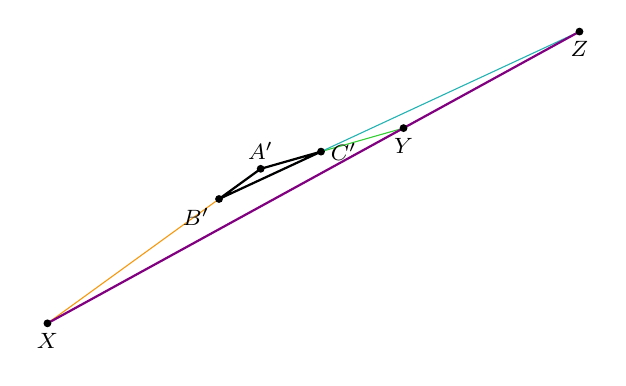
\begin{tikzpicture}[scale=0.06]
    \coordinate (A') at (8.81, 6.384);
    \coordinate (B') at (0, 0);
    \coordinate (C') at (21.585, 10.024);
    \coordinate (X) at (-36.326, -26.326);
    \coordinate (Y) at (39.052, 15);
    \coordinate (Z) at (76.3, 35.433);

    \draw[LimeGreen] (A') -- (Y);
    \draw[TealBlue] (B') -- (Z);
    \draw[YellowOrange] (X) -- (A');

    \draw[thick, violet] (X) -- (Z);

    \draw[thick] (A') -- (B') -- (C') -- (A');

    \foreach \n in {A', B', C', X, Y, Z}
        \node at (\n)[circle,fill,inner sep=1pt]{};

    \node[above] at (A') {\footnotesize $A'$};
    \node[below left] at (B') {\footnotesize $B'$};
    \node[right] at (C') {\footnotesize $C'$};
    \node[below] at (X) {\footnotesize $X$};
    \node[below] at (Y) {\footnotesize $Y$};
    \node[below] at (Z) {\footnotesize $Z$};
\end{tikzpicture}
\end{center}

By converse of Menelaus' Theorem, it is evident that $X$, $Y$, and
$Z$ are collinear.

Now that the first statement for if and only if condition is proven,
the converse must also be proven. Consider the diagram below where the
same construction method is used. Note that if $AA'$, $BB'$, and $CC'$
concur is yet to be known.

\begin{center}
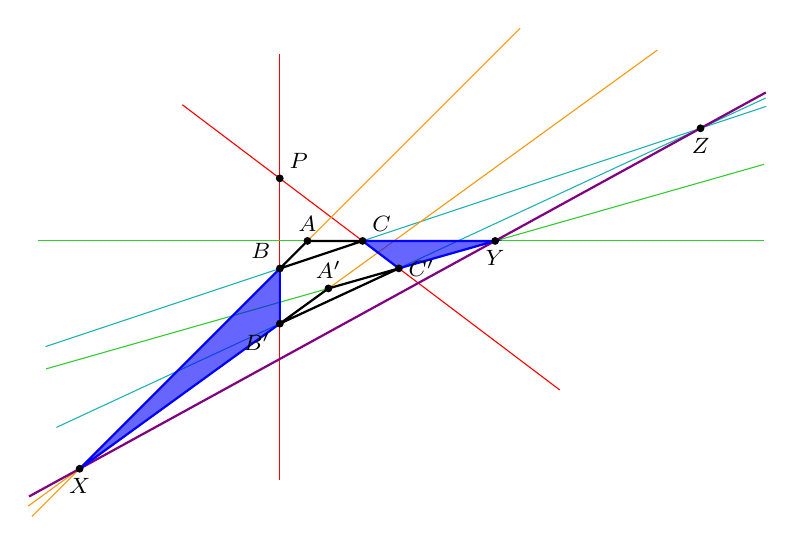
\begin{tikzpicture}[scale=0.07]
    \coordinate (A) at (5, 15);
    \coordinate (B) at (0, 10);
    \coordinate (C) at (15, 15);
    \coordinate (A') at (8.81, 6.384);
    \coordinate (B') at (0, 0);
    \coordinate (C') at (21.585, 10.024);
    \coordinate (P) at (-0.018, 26.349);
    \coordinate (X) at (-36.326, -26.326);
    \coordinate (Y) at (39.052, 15);
    \coordinate (Z) at (76.3, 35.433);

    \draw[red] (-17.695, 39.707) -- (50.757, -12.021);
    \draw[red] (0, 48.926) -- (0, -28.305);

    \draw[LimeGreen] (-43.959, 15) -- (87.893, 15);
    \draw[LimeGreen] (-42.399, -8.204) -- (87.824, 28.894);
    \draw[TealBlue] (-42.509, -4.17) -- (88.226, 39.409);
    \draw[TealBlue] (-40.544, -18.828) -- (88.117, 40.921);
    \draw[YellowOrange]
        (-45.653, -33.086) -- (68.479, 49.628);
    \draw[YellowOrange]
        (-45, -35) -- (43.588, 53.588);

    \draw[thick, violet]
        (-45.498, -31.355) -- (88.156, 41.935);

    \draw[thick] (A) -- (B) -- (C) -- (A);
    \draw[thick] (A') -- (B') -- (C') -- (A');
    \draw[thick, blue] (B) -- (B') -- (X) -- (B);
    \draw[thick, blue] (C) -- (C') -- (Y) -- (C);

    \fill[blue, opacity=0.6] (B) -- (B') -- (X);
    \fill[blue, opacity=0.6] (C) -- (C') -- (Y);

    \foreach \n in {A, B, C, A', B', C', X, Y, Z, P}
        \node at (\n)[circle,fill,inner sep=1pt]{};

    \node[above] at (A) {\footnotesize $A$};
    \node[above left] at (B) {\footnotesize $B$};
    \node[above right] at (C) {\footnotesize $C$};
    \node[above] at (A') {\footnotesize $A'$};
    \node[below left] at (B') {\footnotesize $B'$};
    \node[right] at (C') {\footnotesize $C'$};
    \node[above right] at (P) {\footnotesize $P$};
    \node[below] at (X) {\footnotesize $X$};
    \node[below] at (Y) {\footnotesize $Y$};
    \node[below] at (Z) {\footnotesize $Z$};
\end{tikzpicture}
\end{center}

Notice that $\triangle{XBB'}$ and $\triangle{YCC'}$ are in
perspective from point $Z$. Moreover, the first half of the proof
manifests that $P$, $A$, and $A'$ must be collinear. By construction,
$P$ is on line $BB'$ and $CC'$. Moreover, it is also on the line
$AA'$. Thus, $\triangle{ABC}$ and $\triangle{A'B'C'}$ are centrally
perspective if they are axially perspective.
\end{proof}

This is it for the proof! Before we move on to the next problem,
let's solve a quick example problem.

\begin{problem}{}{}
$D$ is a point on $\overline{BC}$ in $\triangle{ABC}$. Let $I_1$,
$I_2$ be the incenter of $\triangle{ABD}$ and $\triangle{ACD}$
respectively. Moreover, let $I_3$ and $I_4$ be ex-centers in
respect to $\angle{BAD}$ and $\angle{CAD}$ respectively. Show that
$\overline{I_1 I_2}$, $\overline{I_3 I_4}$, and $\overline{BC}$
intersect at one point.
\end{problem}
(\href{https://www.youtube.com/watch?v=adwiSgEAIG0}{Video Solution})
\begin{proof}
First, because $I_1$ and $I_2$ are the angle bisectors of
$\angle{ABD}$ and $\angle{ACD}$ respectively, $I = BI_1 \cap CI_2$
is the incenter of $\triangle{ABC}$. Similarly, we know that $I' =
BI_3 \cap CI_4$ is the ex-center of $\triangle{ABC}$ in respect that
$\angle{BAC}$. Therefore $A$, $I$, and $I'$ are collinear.

With similar idea, we could prove that $A, I_1, I_3$ are collinear
as well as $A, I_2, I_4$. In other words, $I_1I_3$ and $I_2I_4$
intersect at point $A$. Therefore, $BI_1 \cap CI_2$, $I_1I_3 \cap
I_2I_4$, and $I_3B \cap I_4C$ are collinear in $\triangle{I_1BI_3}$
and $\triangle{I_2CI_4}$. By Desargues' theorem, $\overline{I_1 I_2}$,
$\overline{I_3 I_4}$, and $\overline{BC}$ concurs.
\end{proof}



\end{document}


